\documentclass[aspectratio=169, 10pt]{beamer}

% ---------- Tema y colores ----------
\usetheme{default}
\usecolortheme{default}
\setbeamertemplate{navigation symbols}{}
\setbeamertemplate{footline}[frame number]
\setbeamertemplate{frametitle continuation}{}

\definecolor{StanfordRed}{RGB}{140,21,21}
\definecolor{StanfordGray}{RGB}{77,77,77}
\definecolor{LightGray}{RGB}{240,240,240}
\definecolor{AccentBlue}{RGB}{0,84,166}
\definecolor{AccentGreen}{RGB}{0,130,100}
\definecolor{UCMBlue}{RGB}{4, 171, 226}
\definecolor{UCMNavy}{RGB}{20, 65, 134}

\setbeamercolor{frametitle}{fg=white, bg=UCMBlue}
\setbeamercolor{title}{fg=white}
\setbeamercolor{author}{fg=white}
\setbeamercolor{institute}{fg=white!80}
\setbeamercolor{structure}{fg=UCMBlue}
\setbeamercolor{block title}{bg=UCMBlue!15!white, fg=UCMBlue}
\setbeamercolor{block body}{bg=LightGray}
\setbeamercolor{alerted text}{fg=UCMBlue}
\setbeamercolor{example text}{fg=UCMBlue}

\setbeamerfont{frametitle}{series=\bfseries, size=\large}
\setbeamerfont{title}{series=\bfseries, size=\LARGE}
\setbeamerfont{block title}{series=\bfseries}

% ---------- Paquetes ----------
\usepackage[utf8]{inputenc}
\usepackage[T1]{fontenc}
\usepackage[provide=*,spanish]{babel}
\usepackage{amsmath, amssymb, bm}
\usepackage{algorithmic}
\usepackage{tikz}
\usepackage{pgfplots}
\pgfplotsset{compat=1.18}
\usetikzlibrary{arrows.meta, shapes.geometric, positioning, fit, calc,
	decorations.pathreplacing, backgrounds, shadows, patterns}
\usepackage{booktabs}
\usepackage{xcolor}
\usepackage{multicol}
\usepackage{tcolorbox}
\tcbuselibrary{skins, breakable}

% ---------- Comandos útiles ----------
\newcommand{\R}{\mathbb{R}}
\newcommand{\E}{\mathbb{E}}
\newcommand{\gv}{\bm{g}}
\newcommand{\xv}{\bm{x}}
\newcommand{\dv}{\bm{d}}
\newcommand{\vv}{\bm{v}}
\newcommand{\sv}{\bm{s}}
\newcommand{\Amat}{\bm{A}}
\newcommand{\grad}{\nabla}

\newcommand{\formula}[1]{%
	\begin{tcolorbox}[colback=UCMBlue!8, colframe=UCMBlue, arc=4pt,
		boxsep=2pt, left=6pt, right=6pt, top=3pt, bottom=3pt]
		#1
	\end{tcolorbox}
}

% ---------- Portada ----------
\title{\textbf{Optimizaci\'on para Redes Neuronales}}
\subtitle{M\'etodos de primer orden y descenso de gradiente}
\author{Sergio Hern\'andez\\ shernandez@ucm.cl}
\institute{
	% --- Para restaurar el logo institucional, reemplace este tikzpicture por:
	% \includegraphics[width=4cm, height=2cm]{figures/mindslab.png}
	\begin{tikzpicture}[scale=0.42, every node/.style={transform shape}]
		\foreach \i/\y in {1/0,2/1,3/2}{\node[circle,draw=white,fill=white!20,minimum size=4mm] (i\i) at (0,\y){};}
		\foreach \i/\y in {1/-0.5,2/0.5,3/1.5,4/2.5}{\node[circle,draw=white,fill=white!35,minimum size=4mm] (h\i) at (2,\y){};}
		\foreach \i/\y in {1/0.5,2/1.5}{\node[circle,draw=white,fill=white!50,minimum size=4mm] (o\i) at (4,\y){};}
		\foreach \a in {1,2,3}\foreach \b in {1,2,3,4}{\draw[white,opacity=0.5] (i\a)--(h\b);}
		\foreach \a in {1,2,3,4}\foreach \b in {1,2}{\draw[white,opacity=0.5] (h\a)--(o\b);}
	\end{tikzpicture}
	\\ \textbf{Universidad Cat\'olica del Maule}}
\date{}


\begin{document}
% --- Título ---
{
	\setbeamertemplate{background}{
		\begin{tikzpicture}[remember picture, overlay]
			\fill[UCMBlue] (current page.south west) rectangle (current page.north east);
			\fill[UCMBlue!70!black, opacity=0.5]
			(current page.south west) -- ++(0,3) -- ++(18,0) -- cycle;
			\foreach \i in {1,...,40}{
				\fill[white, opacity=0.04]
				({random()*17}, {random()*10}) circle ({random()*0.3});
			}
		\end{tikzpicture}
	}
	\begin{frame}[plain]
		\vspace{1.2cm}
		\titlepage
		\begin{tikzpicture}[remember picture, overlay]
			\node[white, opacity=0.15, font=\fontsize{80}{80}\selectfont]
			at (current page.east) [xshift=-2cm] {$\grad$};
		\end{tikzpicture}
	\end{frame}
}


%=====================================================================
\section{Optimizaci\'on y aprendizaje profundo}
%=====================================================================

\begin{frame}
\frametitle{El problema de optimizaci\'on en deep learning}
Entrenar una red es \textbf{minimizar} una funci\'on de p\'erdida respecto de los par\'ametros $\xv$ (pesos y sesgos):
\formula{\[
\min_{\xv}\; f(\xv), \qquad f(\xv)=\frac{1}{n}\sum_{i=1}^{n}\ell\big(\hat{y}_i(\xv),\,y_i\big).
\]}
\pause
\begin{block}{Dos objetivos que no coinciden}
La \textbf{optimizaci\'on} busca minimizar el error sobre los datos de \emph{entrenamiento}; el \textbf{aprendizaje} busca minimizar el error de \emph{generalizaci\'on}. Reducir uno no garantiza reducir el otro.
\end{block}
\pause
\begin{itemize}
	\item En general $f$ es \textbf{no convexa} y de muy alta dimensi\'on (millones de par\'ametros).
	\item No buscamos el \'optimo global exacto: basta una soluci\'on suficientemente buena, obtenida r\'apido.
\end{itemize}
\end{frame}

\begin{frame}
\frametitle{Desaf\'ios de la optimizaci\'on no convexa}
\begin{columns}[T]
\begin{column}{6.3cm}
\begin{itemize}
	\item \textbf{M\'inimos locales}: un punto mejor que sus vecinos, pero no el mejor global.
	\item \textbf{Puntos de silla}: gradiente nulo que no es ni m\'aximo ni m\'inimo; abundan en alta dimensi\'on.
	\item \textbf{Regiones planas}: gradiente diminuto $\Rightarrow$ avance lento (gradientes que se desvanecen).
\end{itemize}
\end{column}
\begin{column}{5.7cm}
\begin{center}
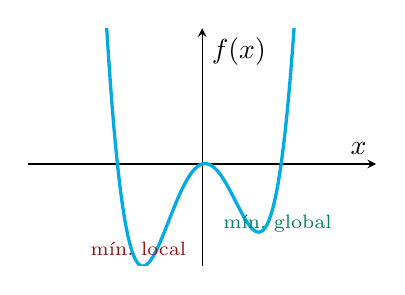
\begin{tikzpicture}
\begin{axis}[width=6cm,height=4.6cm,axis lines=middle,xlabel=$x$,ylabel={$f(x)$},xmin=-3,xmax=3,ymin=-1.2,ymax=1.6,xtick=\empty,ytick=\empty,tick label style={font=\scriptsize}]
\addplot[UCMBlue,very thick,domain=-3:3,samples=200]{x^4-2*x^2+0.2*x};
\node[StanfordRed,font=\scriptsize] at (axis cs:-1.1,-1.0){m\'in. local};
\node[AccentGreen,font=\scriptsize] at (axis cs:1.3,-0.7){m\'in. global};
\end{axis}
\end{tikzpicture}
\end{center}
\end{column}
\end{columns}
\vspace{0.3em}
\footnotesize En la pr\'actica, los m\'etodos de primer orden funcionan sorprendentemente bien pese a estos obst\'aculos: muchos m\'inimos locales en redes grandes tienen p\'erdidas similares.
\end{frame}

\begin{frame}
\frametitle{Convexidad: el caso ideal}
\begin{block}{Funci\'on convexa}
$f$ es convexa si para todo $\lambda\in[0,1]$:
\(\, f\big(\lambda \xv_1 + (1-\lambda)\xv_2\big) \le \lambda f(\xv_1) + (1-\lambda) f(\xv_2).\)
El segmento entre dos puntos del grafo nunca queda por debajo de la curva.
\end{block}
\begin{itemize}
	\item En problemas convexos, \emph{todo} m\'inimo local es global: la optimizaci\'on es ``f\'acil''.
	\pause
	\item Las redes neuronales son \textbf{no convexas}, pero la intuici\'on convexa gu\'ia el dise\~no de los algoritmos.
	\pause
	\item Herramientas clave que reutilizaremos: la \textbf{serie de Taylor de primer orden} y el \textbf{gradiente}.
\end{itemize}
\end{frame}

%=====================================================================
\section{Descenso de gradiente}
%=====================================================================

\begin{frame}
\frametitle{Descenso de gradiente: la direcci\'on de m\'aximo descenso}
Definimos el gradiente en la iteraci\'on $k$ como $\gv^{(k)}=\grad f\big(\xv^{(k)}\big)$. La aproximaci\'on de Taylor de primer orden de un paso de tama\~no $\alpha$ en direcci\'on $\dv$ es:
\formula{\[
f\big(\xv^{(k)} + \alpha\,\dv\big) \approx f\big(\xv^{(k)}\big) + \alpha\,\dv^{\top}\gv^{(k)}.
\]}
\pause
\begin{itemize}
	\item Para reducir $f$ tanto como sea posible (con $\|\dv\|=1$), elegimos la direcci\'on \textbf{opuesta al gradiente}:
	\formula{\[ \dv^{(k)} = -\frac{\gv^{(k)}}{\|\gv^{(k)}\|}. \]}
	\pause
	\item Siguiendo esa direcci\'on, con $\alpha$ suficientemente peque\~no y gradiente no nulo, el avance \emph{garantiza} mejora.
	\item Un punto con gradiente cero es un \textbf{punto estacionario}.
\end{itemize}
\end{frame}

\begin{frame}
\frametitle{Algoritmo de descenso de gradiente}
\begin{algorithmic}[1]
\STATE \textbf{Entrada:} funci\'on $f$, gradiente $\grad f$, punto inicial $\xv^{(1)}$, tasa $\alpha$.
\FOR{$k = 1, 2, \ldots$ hasta convergencia}
  \STATE Calcular el gradiente $\gv^{(k)} = \grad f\big(\xv^{(k)}\big)$.
  \STATE Actualizar $\xv^{(k+1)} = \xv^{(k)} - \alpha\,\gv^{(k)}$.
\ENDFOR
\STATE \textbf{Devolver} $\xv^{(k)}$.
\end{algorithmic}
\vspace{0.8em}
\begin{itemize}
	\item La \textbf{tasa de aprendizaje} $\alpha$ es el hiperpar\'ametro m\'as delicado:
	\begin{itemize}
		\item demasiado peque\~na $\Rightarrow$ convergencia lent\'isima;
		\item demasiado grande $\Rightarrow$ oscilaciones o divergencia.
	\end{itemize}
	\pause
	\item Sin normalizar la direcci\'on, $\alpha$ no corresponde a la longitud real del paso.
\end{itemize}
\end{frame}

\begin{frame}
\frametitle{El problema de los valles estrechos}
\begin{columns}[T]
\begin{column}{6cm}
\begin{itemize}
	\item Si optimizamos el paso en cada iteraci\'on (\emph{line search} exacta), la nueva direcci\'on resulta \textbf{ortogonal} a la anterior:
	\[ \dv^{(k+1)\top}\dv^{(k)} = 0. \]
	\pause
	\item Esto produce trayectorias en \textbf{zig-zag} en valles alargados (p.~ej. la funci\'on de Rosenbrock).
	\pause
	\item El descenso de gradiente puro es sensible al \textbf{escalamiento} de las variables.
\end{itemize}
\end{column}
\begin{column}{6cm}
\begin{center}
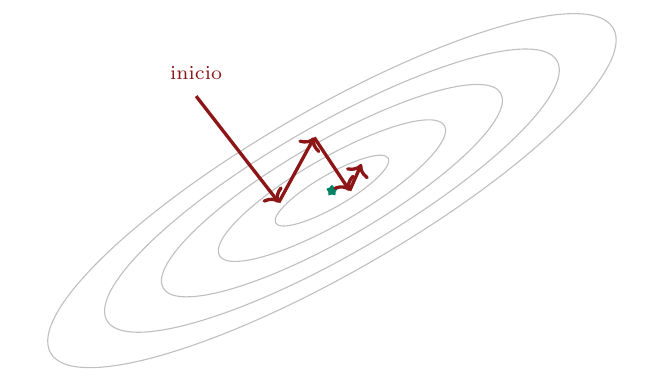
\begin{tikzpicture}[scale=0.75]
\foreach \r in {0.5,1.0,1.5,2.0,2.5}{
	\draw[gray!50,rotate=30] (0,0) ellipse ({2.2*\r} and {0.55*\r});
}
\node[AccentGreen,star,star points=5,fill=AccentGreen,inner sep=1pt] at (0,0) {};
\coordinate (p0) at (-2.3,1.6);
\coordinate (p1) at (-0.9,-0.2);
\coordinate (p2) at (-0.3,0.9);
\coordinate (p3) at (0.3,0.0);
\coordinate (p4) at (0.5,0.45);
\draw[StanfordRed,very thick,->] (p0)--(p1);
\draw[StanfordRed,very thick,->] (p1)--(p2);
\draw[StanfordRed,very thick,->] (p2)--(p3);
\draw[StanfordRed,very thick,->] (p3)--(p4);
\node[StanfordRed,font=\scriptsize] at (-2.3,2.0){inicio};
\end{tikzpicture}
\end{center}
\footnotesize Curvas de nivel de un valle estrecho y el zig-zag del descenso de gradiente.
\end{column}
\end{columns}
\end{frame}

%=====================================================================
\section{Descenso de gradiente estoc\'astico}
%=====================================================================

\begin{frame}
\frametitle{Descenso de gradiente estoc\'astico (SGD)}
\begin{itemize}
	\item El gradiente completo $\grad f(\xv)=\frac{1}{n}\sum_i \grad \ell_i(\xv)$ cuesta $O(n)$ por paso: inviable con millones de ejemplos.
	\pause
	\item \textbf{SGD}: en cada paso se toma un \'unico ejemplo $i$ al azar y se usa su gradiente como \emph{estimador insesgado}:
	\formula{\[ \xv^{(k+1)} = \xv^{(k)} - \alpha\,\grad \ell_i\big(\xv^{(k)}\big), \qquad \E\big[\grad \ell_i(\xv)\big] = \grad f(\xv). \]}
	\pause
	\item Cada paso es $n$ veces m\'as barato, pero el gradiente es \textbf{ruidoso}: la trayectoria fluct\'ua.
	\pause
	\item El ruido puede \emph{ayudar} a escapar de m\'inimos locales pobres y puntos de silla.
	\item Conviene \textbf{reducir} $\alpha$ con el tiempo para amortiguar el ruido cerca del \'optimo.
\end{itemize}
\end{frame}

\begin{frame}
\frametitle{Minibatch SGD: el compromiso pr\'actico}
\begin{itemize}
	\item Un punto intermedio entre el gradiente completo y SGD puro: usar un \textbf{minibatch} $\mathcal{B}$ de $|\mathcal{B}|=b$ ejemplos.
	\formula{\[ \xv^{(k+1)} = \xv^{(k)} - \frac{\alpha}{b}\sum_{i\in\mathcal{B}} \grad \ell_i\big(\xv^{(k)}\big). \]}
	\pause
	\item \textbf{Ventajas}:
	\begin{itemize}
		\item Reduce la varianza del gradiente por un factor $\approx 1/b$.
		\item Aprovecha el paralelismo del hardware (GPU): multiplicaciones matriciales eficientes.
	\end{itemize}
	\pause
	\item El tama\~no de lote $b$ es un compromiso entre \emph{eficiencia computacional} y \emph{calidad del gradiente}; valores t\'ipicos: $32$ a $512$.
	\item Es el caballo de batalla del entrenamiento moderno; todo lo que sigue se construye sobre \'el.
\end{itemize}
\end{frame}

%=====================================================================
\section{Gradiente conjugado}
%=====================================================================

\begin{frame}
\frametitle{Gradiente conjugado: superar los valles}
Inspirado en la optimizaci\'on de funciones cuadr\'aticas $\;\tfrac{1}{2}\xv^{\top}\Amat\xv + \bm{b}^{\top}\xv + c$, con $\Amat$ sim\'etrica y definida positiva.
\begin{itemize}
	\item Genera direcciones \textbf{mutuamente conjugadas} respecto de $\Amat$:
	\formula{\[ \dv^{(i)\top}\Amat\,\dv^{(j)} = 0 \quad \text{para todo } i\neq j. \]}
	\pause
	\item Converge en a lo sumo $n$ pasos en un problema cuadr\'atico de dimensi\'on $n$.
	\pause
	\item Cada direcci\'on combina el gradiente actual con la direcci\'on anterior:
	\formula{\[ \dv^{(k)} = -\gv^{(k)} + \beta^{(k)}\,\dv^{(k-1)}. \]}
	un $\beta^{(k)}$ mayor da m\'as peso a la direcci\'on previa.
\end{itemize}
\end{frame}



%=====================================================================
\section{Momentum}
%=====================================================================

\begin{frame}
\frametitle{Momentum: acumular inercia}
\begin{columns}[T]
\begin{column}{6.3cm}
\begin{itemize}
	\item En regiones casi planas, el gradiente es peque\~no y el avance es lento.
	\item \textbf{Momentum} acumula una \emph{velocidad} $\vv$ que promedia los gradientes recientes:
	\formula{\[
	\begin{aligned}
	\vv^{(k+1)} &= \beta\,\vv^{(k)} - \alpha\,\gv^{(k)},\\
	\xv^{(k+1)} &= \xv^{(k)} + \vv^{(k+1)}.
	\end{aligned}
	\]}
	\item Con $\beta=0$ se recupera el descenso de gradiente.
\end{itemize}
\end{column}
\begin{column}{5.7cm}
\begin{center}
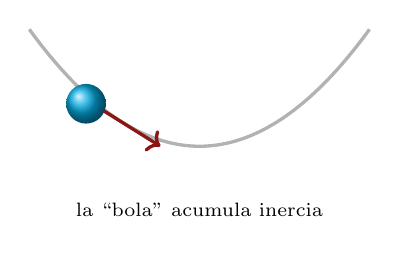
\begin{tikzpicture}[scale=0.9]
\draw[gray!60,very thick] (-2.4,2.0) .. controls (-0.8,-0.2) and (0.8,-0.2) .. (2.4,2.0);
\shade[ball color=UCMBlue] (-1.6,0.95) circle (0.28);
\draw[StanfordRed,very thick,->] (-1.35,0.85) -- (-0.55,0.35);
\node[font=\scriptsize] at (0,-0.55){la ``bola'' acumula inercia};
\end{tikzpicture}
\end{center}
\footnotesize Interpretaci\'on f\'isica: una bola que rueda cuesta abajo gana velocidad; el gradiente actua como la gravedad.
\end{column}
\end{columns}
\pause
\vspace{0.2em}
\begin{block}{}
El momentum suaviza el zig-zag: cancela las componentes oscilatorias y refuerza la direcci\'on consistente hacia el valle.
\end{block}
\end{frame}

\begin{frame}
\frametitle{Momentum de Nesterov}
\begin{itemize}
	\item Problema del momentum cl\'asico: no frena lo suficiente al fondo del valle y tiende a \emph{sobrepasarlo}.
	\pause
	\item \textbf{Nesterov}: evaluar el gradiente en la \textbf{posici\'on futura proyectada} $\xv^{(k)}+\beta\vv^{(k)}$, no en la actual.
	\formula{\[
	\begin{aligned}
	\vv^{(k+1)} &= \beta\,\vv^{(k)} - \alpha\,\grad f\big(\xv^{(k)} + \beta\,\vv^{(k)}\big),\\
	\xv^{(k+1)} &= \xv^{(k)} + \vv^{(k+1)}.
	\end{aligned}
	\]}
	\pause
	\item Es una \emph{correcci\'on anticipada}: ``mira hacia d\'onde voy'' antes de calcular el ajuste.
	\item En la pr\'actica reduce el sobrepaso y suele converger algo m\'as r\'apido que el momentum cl\'asico.
\end{itemize}
\end{frame}

%=====================================================================
\section{M\'etodos de tasa adaptativa}
%=====================================================================

\begin{frame}
\frametitle{AdaGrad: una tasa por par\'ametro}
Momentum aplica la misma tasa a todas las componentes. \textbf{AdaGrad} adapta una tasa para \emph{cada} par\'ametro $x_i$ seg\'un su historial de gradientes.
\formula{\[
s_i^{(k)} = \sum_{j=1}^{k}\big(g_i^{(j)}\big)^2,
\qquad
x_i^{(k+1)} = x_i^{(k)} - \frac{\alpha}{\epsilon + \sqrt{s_i^{(k)}}}\,g_i^{(k)}.
\]}
\begin{itemize}
	\item Par\'ametros con gradientes grandes reciben pasos m\'as peque\~nos, y viceversa: \'util con gradientes \textbf{dispersos}.
	\item Poco sensible a la tasa base (a menudo $\alpha=0.01$); $\epsilon\sim 10^{-8}$ evita dividir por cero.
	\pause
	\item \textbf{Debilidad}: $s_i$ s\'olo crece $\Rightarrow$ la tasa efectiva decae mon\'otonamente y puede volverse \emph{infinitesimal} antes de converger.
\end{itemize}
\end{frame}

\begin{frame}
\frametitle{RMSProp y Adadelta: corregir el decaimiento}
\begin{columns}[T]
\begin{column}{6cm}
\textbf{RMSProp}
\begin{itemize}
	\item Reemplaza la suma acumulada por una \textbf{media m\'ovil} con decaimiento $\gamma\approx 0.9$:
\end{itemize}
\formula{\[
\hat{s}^{(k+1)} = \gamma\,\hat{s}^{(k)} + (1-\gamma)\big(\gv^{(k)}\odot\gv^{(k)}\big)
\]}
\[ x_i^{(k+1)} = x_i^{(k)} - \frac{\alpha}{\epsilon+\sqrt{\hat{s}_i^{(k+1)}}}\,g_i^{(k)} \]
La tasa efectiva ya no decae sin l\'imite.
\end{column}
\begin{column}{6cm}
\textbf{Adadelta}
\begin{itemize}
	\item Tambi\'en evita el decaimiento mon\'otono, y adem\'as \textbf{elimina} la tasa $\alpha$.
	\item Usa una media m\'ovil de los \emph{cuadrados de las actualizaciones} para corregir las unidades:
\end{itemize}
\formula{\[
x_i^{(k+1)} = x_i^{(k)} - \frac{\mathrm{RMS}(\Delta x_i)}{\epsilon+\mathrm{RMS}(g_i)}\,g_i^{(k)}
\]}
\end{column}
\end{columns}
\vspace{0.5em}
\footnotesize $\odot$ es el producto elemento a elemento; $\mathrm{RMS}$ denota la ra\'iz cuadr\'atica media con decaimiento.
\end{frame}

\begin{frame}
\frametitle{Adam: momentum + tasa adaptativa}
\textbf{Adam} combina un promedio decreciente del gradiente (como momentum) y de su cuadrado (como RMSProp), con \emph{correcci\'on de sesgo} inicial.
\begin{align*}
\vv^{(k+1)} &= \gamma_v\,\vv^{(k)} + (1-\gamma_v)\,\gv^{(k)} & \text{(1\textsuperscript{er} momento)}\\
\sv^{(k+1)} &= \gamma_s\,\sv^{(k)} + (1-\gamma_s)\big(\gv^{(k)}\odot\gv^{(k)}\big) & \text{(2\textsuperscript{do} momento)}\\
\hat{\vv}^{(k+1)} &= \vv^{(k+1)}/(1-\gamma_v^{\,k}), \qquad
\hat{\sv}^{(k+1)} = \sv^{(k+1)}/(1-\gamma_s^{\,k}) & \text{(correcci\'on)}\\
\xv^{(k+1)} &= \xv^{(k)} - \alpha\,\hat{\vv}^{(k+1)} \big/ \big(\epsilon + \sqrt{\hat{\sv}^{(k+1)}}\big) & \text{(actualizaci\'on)}
\end{align*}
\pause
\begin{block}{Valores por defecto (paper original)}
$\alpha=0.001$, \quad $\gamma_v=0.9$, \quad $\gamma_s=0.999$, \quad $\epsilon=10^{-8}$. Es el optimizador m\'as usado por defecto en deep learning.
\end{block}
\end{frame}

\begin{frame}
\frametitle{Comparaci\'on de optimizadores}
\begin{center}
\begin{tabular}{lll}
\toprule
\textbf{M\'etodo} & \textbf{Idea a\~nadida} & \textbf{Hiperpar\'ametros}\\
\midrule
SGD              & Gradiente ruidoso por minibatch & $\alpha$\\
Momentum         & Inercia / velocidad acumulada   & $\alpha,\beta$\\
Nesterov         & Gradiente en posici\'on proyectada & $\alpha,\beta$\\
AdaGrad          & Tasa por par\'ametro (suma de $g^2$) & $\alpha$\\
RMSProp          & Media m\'ovil de $g^2$           & $\alpha,\gamma$\\
Adadelta         & RMSProp sin tasa $\alpha$        & $\gamma_s,\gamma_x$\\
Adam             & Momentum $+$ RMSProp $+$ correcci\'on & $\alpha,\gamma_v,\gamma_s$\\
\bottomrule
\end{tabular}
\end{center}
\vspace{0.8em}
\begin{itemize}
	\item \textbf{Punto de partida razonable}: Adam (r\'apido y robusto) o SGD con momentum (suele generalizar muy bien con buen ajuste).
\end{itemize}
\end{frame}

%=====================================================================
\section{Tasa de aprendizaje e hipergradiente}
%=====================================================================

\begin{frame}
\frametitle{Programaci\'on de la tasa de aprendizaje}
\begin{columns}[T]
\begin{column}{5.6cm}
\begin{itemize}
	\item Mantener $\alpha$ fija rara vez es \'optimo: conviene \textbf{variarla} durante el entrenamiento.
	\item Esquemas comunes:
	\begin{itemize}
		\item \emph{Decaimiento por escalones}.
		\item \emph{Decaimiento coseno}.
		\item \emph{Calentamiento} (\emph{warmup}) inicial.
	\end{itemize}
	\item Empezar alto (avanzar r\'apido) y bajar (asentarse en el m\'inimo) suele dar lo mejor de ambos mundos.
\end{itemize}
\end{column}
\begin{column}{6.4cm}
\begin{center}
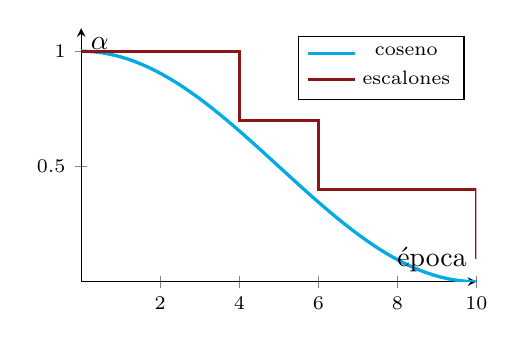
\begin{tikzpicture}
\begin{axis}[width=6.6cm,height=4.8cm,axis lines=middle,xlabel={\'epoca},ylabel={$\alpha$},xmin=0,xmax=10,ymin=0,ymax=1.1,legend pos=north east,tick label style={font=\scriptsize},legend style={font=\scriptsize}]
\addplot[UCMBlue,very thick,domain=0:10,samples=200]{0.5*(1+cos(deg(pi*x/10)))};
\addplot[StanfordRed,very thick,const plot,domain=0:10,samples=6]{1-floor(x/3)*0.3};
\legend{coseno,escalones}
\end{axis}
\end{tikzpicture}
\end{center}
\end{column}
\end{columns}
\end{frame}

\begin{frame}
\frametitle{Descenso por hipergradiente}
\begin{itemize}
	\item Los m\'etodos acelerados son muy sensibles a la tasa $\alpha$, o gastan mucho esfuerzo en adaptarla.
	\pause
	\item Idea: aplicar \emph{descenso de gradiente a la propia tasa}. Un \textbf{hipergradiente} es la derivada de $f$ respecto de un hiperpar\'ametro.
	\pause
	\item Para el descenso de gradiente, la derivada respecto de $\alpha$ resulta:
	\formula{\[
	\frac{\partial f\big(\xv^{(k+1)}\big)}{\partial \alpha^{(k)}}
	= \gv^{(k+1)\top}\big(-\gv^{(k)}\big),
	\qquad
	\alpha^{(k)} = \alpha^{(k-1)} + \mu\,\gv^{(k)\top}\gv^{(k-1)}.
	\]}
	\pause
	\item S\'olo requiere recordar el gradiente anterior; reduce la sensibilidad a la elecci\'on inicial de $\alpha$.
\end{itemize}
\end{frame}

%=====================================================================
\section{Resumen}
%=====================================================================

\begin{frame}
\frametitle{Resumen}
\begin{itemize}
	\item El \textbf{descenso de gradiente} sigue la direcci\'on de m\'aximo descenso; su tasa de aprendizaje es cr\'itica.
	\item \textbf{SGD / minibatch} hacen viable el entrenamiento a gran escala a costa de gradientes ruidosos.
	\item El \textbf{gradiente conjugado} se adapta a los valles locales reutilizando informaci\'on previa.
	\item El \textbf{momentum} (y Nesterov) acumula progreso en direcciones favorables y suaviza el zig-zag.
	\item Los m\'etodos de \textbf{tasa adaptativa} (AdaGrad, RMSProp, Adadelta, \textbf{Adam}) ajustan el paso por par\'ametro.
	\item La \textbf{programaci\'on de la tasa} y el \textbf{hipergradiente} reducen la dependencia del ajuste manual.
\end{itemize}
\vspace{0.4em}
\begin{block}{}
No existe un optimizador \'unico ``mejor'': la elecci\'on depende del problema, los datos y el presupuesto de c\'omputo.
\end{block}
\end{frame}

\begin{frame}
\frametitle{Para profundizar}
\begin{itemize}
	\item Zhang, Lipton, Li \& Smola, \emph{Dive into Deep Learning}, cap.~12 (Optimization Algorithms)\\ \url{https://d2l.ai/chapter_optimization/index.html}
	\item Kochenderfer \& Wheeler, \emph{Algorithms for Optimization}, cap.~5 (First-Order Methods), MIT Press.
	\item Goodfellow, Bengio \& Courville, \emph{Deep Learning}, cap.~8 (Optimization for Training Deep Models).
	\item Kingma \& Ba (2015), \emph{Adam: A Method for Stochastic Optimization}, ICLR.
	\item Duchi, Hazan \& Singer (2011), \emph{Adaptive Subgradient Methods} (AdaGrad), JMLR.
	\item Nesterov (1983); Baydin et al.\ (2018), \emph{Online Learning Rate Adaptation with Hypergradient Descent}.
\end{itemize}
\end{frame}

\end{document}
